\documentclass[12pt,a4paper]{article}
\usepackage[T2A]{fontenc}
\usepackage[utf8]{inputenc}
\usepackage[russian]{babel}
\usepackage{graphicx, setspace, hyperref, listings}

\usepackage[
top = 1.25cm, 
bottom = 2.0cm]{geometry}

\begin{document}
\begin{titlepage} 
	\centering
    % HEADER
	{
        \scshape
        Федеральное государственное автономное образовательное учреждение высшего образования
        \par
        \textbf{«Научно-образовательная корпорация ИТМО»}
        \par
        \vspace{1cm}
        Факультет Программной Инженерии и Компьютерной Техники
        \par
    }
    % LOGO
    \vspace{0.6cm}
    
\includegraphics[width=\textwidth]{logo.png}
    % LAB INFO
    {
        \Large
        \textbf{Лабораторная работа №2 по основам программной инженерии}
        \par
        \normalsize
        \vspace{0.75cm}
        \textbf{Вариант 99876}
        \par
    }
    \vfill
    % СREDITS
    \hfill\begin{minipage}{\dimexpr\textwidth-7.8cm}
        \textbf{Выполнили:}\par
        Степанов Арсений Алексеевич\par
        Шпак Всеволод Васильевич\par
        \vspace{0.15cm}
        \textbf{Группа:}\par
        P3209\par
        \vspace{0.15cm}
        \textbf{Преподаватель:}\par
        Пименов Данила Дмитриевич\par
    \end{minipage}
    \vfill
    Санкт-Петербург, \the\year{}г
\end{titlepage}  
\section{Задание}
Сконфигурировать в своём домашнем каталоге репозитории svn и git и загрузить в них начальную ревизию файлов с исходными кодами (в соответствии с выданным вариантом)
\\ \hfill \break
Воспроизвести последовательность команд для систем контроля версий svn и git, осуществляющих операции над исходным кодом, приведённые на блок-схеме
\\ \hfill \break
При составлении последовательности команд необходимо учитывать следующие условия:
\begin{itemize}
    \item Цвет элементов схемы указывает на пользователя, совершившего действие (красный - первый, синий - второй)
    \item Цифры над узлами - номер ревизии. Ревизии создаются последовательно
    \item Необходимо разрешать конфликты между версиями, если они возникают
\end{itemize}
\subsection{Схема}
\begin{center}
    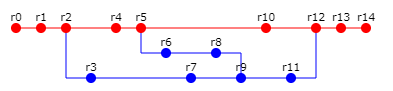
\includegraphics[width=\textwidth]{scheme.png}
\end{center}
\section{Последовательность команд}
\subsection{Для системы Git}
\begin{lstlisting}[language=Bash]
    rm -rf repo_user1 repo_user2

    mkdir repo_user1
    mkdir repo_user2
    
    # User 1
    cd repo_user1
    git init
    cp -rf ../commits/commit0/* .
    git add .
    git commit -m 'r0'
    git branch -M main
    git remote add origin $GIT_REPO
    git push -u origin main
    cp -rf ../commits/commit1/* .
    git add .
    git commit -m 'r1'
    git push -u origin main
    cp -rf ../commits/commit2/* .
    git add .
    git commit -m 'r2'
    git push -u origin main
    
    # User 2
    cd ../repo_user2
    git clone $GIT_REPO .
    git checkout -b branch1
    cp -rf ../commits/commit3/* .
    git add .
    git commit -m 'r3'
    git push --set-upstream origin branch1
    
    # User 1
    cd ../repo_user1
    git pull
    cp -rf ../commits/commit4/* .
    git add .
    git commit -m 'r4'
    git push --set-upstream origin main
    cp -rf ../commits/commit5/* .
    git add .
    git commit -m 'r5'
    git push --set-upstream origin main
    
    # User 2
    cd ../repo_user2
    git pull
    git checkout main
    git checkout -b branch2
    cp -rf ../commits/commit6/* .
    git add .
    git commit -m 'r6'
    git push --set-upstream origin branch2
    git checkout branch1
    cp -rf ../commits/commit7/* .
    git add .
    git commit -m 'r7'
    git push --set-upstream origin branch1
    git checkout branch2
    cp -rf ../commits/commit8/* .
    git add .
    git commit -m 'r8'
    git push --set-upstream origin branch2
    git checkout branch1
    git merge branch2 -m 'branch2 > branch1' 
    git branch -d branch2
    cp -rf ../commits/commit9/* .
    git add .
    git commit -m 'r9'
    git push --set-upstream origin branch1
    
    # User 1
    cd ../repo_user1
    git pull
    cp -rf ../commits/commit10/* .
    git add .
    git commit -m 'r10'
    git push --set-upstream origin main
    
    # User 2
    cd ../repo_user2
    git pull
    cp -rf ../commits/commit11/* .
    git add .
    git commit -m 'r11'
    git push --set-upstream origin branch1
    
    # User 1
    cd ../repo_user1
    git pull
    git merge branch1 -m 'branch1 > main' 
    git branch -d branch1
    cp -rf ../commits/commit12/* .
    git add .
    git commit -m 'r12'
    git push --set-upstream origin main
    cp -rf ../commits/commit13/* .
    git add .
    git commit -m 'r13'
    git push --set-upstream origin main
    cp -rf ../commits/commit14/* .
    git add .
    git commit -m 'r14'
    git push --set-upstream origin main
    
    cd ..
    
\end{lstlisting}
\subsection{Для системы Subversion}
\begin{lstlisting}[language=Bash]
rm -rf repo_user1 repo_user2

mkdir repo_user1 repo_user2

# User 1
cd repo_user1
svn checkout $SVN_REPO .
cp -rf ../commits/commit0/* .
svn add --force .
svn commit -m 'r0' --username $SVN_USERNAME --password $SVN_PASSWORD
cp -rf ../commits/commit1/* .
svn add --force .
svn commit -m 'r1' --username $SVN_USERNAME --password $SVN_PASSWORD
cp -rf ../commits/commit2/* .
svn add --force .
svn commit -m 'r2' --username $SVN_USERNAME --password $SVN_PASSWORD

# User 2
cd ../repo_user2
svn checkout $SVN_REPO .
svn copy $SVN_REPO/trunk $SVN_REPO/branches/branch1 -m 'Create branch1'
svn switch $SVN_REPO/branches/branch1 --ignore-ancestry
cp -rf ../commits/commit3/* .
svn add --force .
svn commit -m 'r3' --username $SVN_USERNAME --password $SVN_PASSWORD

# User 1
cd ../repo_user1
svn update
cp -rf ../commits/commit4/* .
svn add --force .
svn commit -m 'r4' --username $SVN_USERNAME --password $SVN_PASSWORD
cp -rf ../commits/commit5/* .
svn add --force .
svn commit -m 'r5' --username $SVN_USERNAME --password $SVN_PASSWORD

# User 2
cd ../repo_user2
svn update
svn switch $SVN_REPO/branches/branch1 --ignore-ancestry
cp -rf ../commits/commit6/* .
svn add --force .
svn commit -m 'r6' --username $SVN_USERNAME --password $SVN_PASSWORD
svn copy $SVN_REPO/trunk $SVN_REPO/branches/branch2 -m 'Create branch2'
svn switch $SVN_REPO/branches/branch2 --ignore-ancestry
cp -rf ../commits/commit7/* .
svn add --force .
svn commit -m 'r7' --username $SVN_USERNAME --password $SVN_PASSWORD
svn switch $SVN_REPO/branches/branch1 --ignore-ancestry
cp -rf ../commits/commit8/* .
svn add --force .
svn commit -m 'r8' --username $SVN_USERNAME --password $SVN_PASSWORD
svn up
svn merge $SVN_REPO/branches/branch2
svn commit -m 'branch2 > branch1' --username $SVN_USERNAME --password $SVN_PASSWORD
svn delete $SVN_REPO/branches/branch2 -m 'Delete branch2' --username $SVN_USERNAME --password $SVN_PASSWORD
cp -rf ../commits/commit9/* .
svn add --force .
svn commit -m 'r9' --username $SVN_USERNAME --password $SVN_PASSWORD

# User 1
cd ../repo_user1
svn update
cp -rf ../commits/commit10/* .
svn add --force .
svn commit -m 'r10' --username $SVN_USERNAME --password $SVN_PASSWORD
svn switch $SVN_REPO/trunk --ignore-ancestry
svn merge $SVN_REPO/branches/branch1
svn commit -m 'branch1 > main' --username $SVN_USERNAME --password $SVN_PASSWORD
svn delete $SVN_REPO/branches/branch1 -m 'Delete branch1' --username $SVN_USERNAME --password $SVN_PASSWORD
cp -rf ../commits/commit11/* .
svn add --force .
svn commit -m 'r11' --username $SVN_USERNAME --password $SVN_PASSWORD
cp -rf ../commits/commit12/* .
svn add --force .
svn commit -m 'r12' --username $SVN_USERNAME --password $SVN_PASSWORD
cp -rf ../commits/commit13/* .
svn add --force .
svn commit -m 'r13' --username $SVN_USERNAME --password $SVN_PASSWORD
cp -rf ../commits/commit14/* .
svn add --force .
svn commit -m 'r14' --username $SVN_USERNAME --password $SVN_PASSWORD

cd ..
\end{lstlisting}
\section{Вывод}
Мы научились работать с системами контроля версий Git и Svn, ознакомились с основными принципами и базовыми командами
\end{document}